%%%%%%%%%%%%%%%%%%%%%%%%%%%%%%%%%%%%%%%%%%%%%%%%%%%%%%%%%%%%%%%%%%%%%%
%% GABM Tipping Point and Competing Persuasion
%% Methodology paper for pol-sci quants seminar.
%% Single-file source per Springer Nature submission policy.
%%%%%%%%%%%%%%%%%%%%%%%%%%%%%%%%%%%%%%%%%%%%%%%%%%%%%%%%%%%%%%%%%%%%%%

\documentclass[pdflatex,sn-mathphys-num]{sn-jnl}% Numbered references

%%%% Standard Packages
\usepackage{graphicx}%
\usepackage{multirow}%
\usepackage{amsmath,amssymb,amsfonts}%
\usepackage{amsthm}%
\usepackage{mathrsfs}%
\usepackage[title]{appendix}%
\usepackage{xcolor}%
\usepackage{textcomp}%
\usepackage{manyfoot}%
\usepackage{booktabs}%
\usepackage{algorithm}%
\usepackage{algorithmicx}%
\usepackage{algpseudocode}%
\usepackage{listings}%

\theoremstyle{thmstyleone}%
\newtheorem{theorem}{Theorem}%
\newtheorem{proposition}[theorem]{Proposition}%

\theoremstyle{thmstyletwo}%
\newtheorem{example}{Example}%
\newtheorem{remark}{Remark}%

\theoremstyle{thmstylethree}%
\newtheorem{definition}{Definition}%

\raggedbottom

\begin{document}

\title[GABM Framework for Competing Committed Minorities]{
Understanding the dynamics of social tipping with two competing
committed minority groups using a Generative-AI Agent-Based Model Approach}

%%==================== AUTHORS ====================%%
\author*[1]{\fnm{Ajaykumar} \sur{Manivannan}}
\email{a.manivannan@leeds.ac.uk}

\author*[1]{\fnm{Viktoria} \sur{Spaiser}}
\email{V.Spaiser@leeds.ac.uk}

\author[1]{\fnm{Andy} \sur{Turner}}

\author[1]{\fnm{Charlie} \sur{Pilgrim}}

\affil*[1]{
\orgname{University of Leeds},
\orgaddress{\city{Leeds}, \country{United Kingdom}}}

%%==================== ABSTRACT ====================%%
\abstract{%
%Small political groups can shape public debate far beyond their size, but models of this process often strip away the people doing the persuading. 
Committed minorities have been shown to be able to overturn established attitudes or
practices and shift a majority to its viewpoint. However, in real world context a
committed minority rarely acts in isolation and tipping dynamics are less clear if two
opposing committed minorities are attempting to shift a majority.  This paper presents a
generative-AI agent-based model (GABM) of UK climate-policy opinion designed to study
such complex dynamics. Each citizen AI agent is anchored to a real respondent in a
representative YouGov survey, i.e. the simulation starts from observed opinions. Two
committed minority AI agents are loosely modelled on Reform UK and the Green Party,
using persuasive communication drawn from a fixed, curated pool of synthetic messages
for each side, each grounded in the groups' real online communications, to shift the
majority opinion. The AI agents are
placed on a social network,
where they can communicate with each other and allow broadcast from the committed
minority AI agents to the citizen AI agents. Different experiments are run with the GABM
to test how tipping or polarization dynamics unfold if the minority groups have
different resources that allow them to reach a larger share of the majority and/or
communicate their persuasive messages more frequently.
%We report two illustrative probes: a seven-day run under symmetric political broadcasts, and a four-day single-policy run that varies broadcast reach. We also test whether the survey component reads the personas it is given and document where residual bias remains. This is a short methodological note, not a tipping claim. Its purpose is to present the framework, report the first results, and identify the main questions for the next round of work.
}

\keywords{generative agent-based modelling, opinion dynamics, committed minorities, large language models, climate policy, social tipping points, polarization}

\maketitle

%%%%%%%%%%%%%%%%%%%%%%%%%%%%%%%%%%%%%%%%%%%%%%%%%%%%%%%%%%%%%%%%%%%%%%
%% 1. INTRODUCTION
%%%%%%%%%%%%%%%%%%%%%%%%%%%%%%%%%%%%%%%%%%%%%%%%%%%%%%%%%%%%%%%%%%%%%%
\section*{NOTE: INCOMPLETE WORK IN PROGRESS}

\section{Introduction}\label{sec:intro}

%Public opinion on contested policy is rarely uniform, and it is rarely static. Small, organised groups can shape debate well beyond their own size. In this paper, we use the term \emph{committed minorities} for political actors that hold a stable position and keep pressing the same message over time. UK climate politics offers a clear example. Reform UK and the Green Party of England and Wales hold only a small share of seats in Parliament, but their arguments about carbon taxes, petrol cars, renewable energy, and home heating travel well beyond their own voters. A basic question follows: how do such groups shift wider public opinion, and under what conditions does one side gain ground?

LITERATURE REVIEW ON SOCIAL TIPPING, COMMITTED MINORITIES, PERSUASION AND CLIMATE
POLICIES IN THE UK TO BE WRITTEN

Classical models of committed-minority dynamics offer a useful starting point because
they show how a small group can sometimes move a much larger population towards its
viewpoint ~\cite{centola2018, granovetter1978, galam2002}. But they usually model
citizens as simple agents with binary opinion states that follow fixed update rules
rather than respond to communication that may or may not resonate with their values and
goals. Generative-AI agent-based models (GABMs) take a different approach. In a GABM,
agents are built using large language models (LLMs) to generate complex personas that
have socio-demographic background and values and that can communicate, i.e. generate
messages, reflections, and answer surveys~\cite{park2023, tornberg2023,
ghaffarzadegan2024, vezhnevets2023concordia}. This makes it possible to represent richer
personas and arguments, but it also introduces challenges. For instance, LLMs tend to
generate socially favoured responses and hence are less likely to generate varied
opinions when used to answer surveys~\cite{argyle2023, santurkar2023, bisbee2024,
manivannan2026}. %For climate policy, that can make a simulation start from
unrealistically pro-climate views unless the starting point is carefully controlled.
Our GABM of UK climate-policy opinion dynamics therefore anchors each citizen AI agent
to a real respondent in a
representative YouGov survey, i.e. the model is calibrated to real-world data. Two
committed minority AI agents, loosely
modelled on Reform UK and the Green Party, send opposing messages meant to sway the
citizen AI agents. These messages are drawn from a fixed, curated pool for each side;
they are synthetic but each is grounded in the parties' real online climate-policy
communications (party manifestos, parliamentary speeches, and press statements).
Furthermore, citizen AI agents
can share their reflections after being exposed to committed minority communication with
other AI citizens they are connected with on a social network.

The model allows manipulation of various parameters to run experiments aimed at studying
tipping or polarising opinion dynamics. In this paper, we study how opinion dynamics
change when one committed minority has more resources than the other. Crucially, a
resource advantage can take different forms: reaching more citizen AI agents,
broadcasting more frequently, or aiming a limited broadcast more selectively. Classical
committed-minority models collapse these forms into a single abstract influence weight;
because a GABM's agents process natural-language messages against their personas, it can
hold the levers apart and estimate their effects separately. This paper makes two
contributions: (i)~a GABM framework, together with a reusable fit-for-purpose evaluation
protocol, for studying competing committed minorities; and (ii)~a first demonstration
that the form of a resource asymmetry, not merely its magnitude, shapes which
side moves the majority, and that the forms are not interchangeable. We are careful
about the epistemic status of these results: we make no claim that the model reproduces
real-world opinion dynamics, and our evidence targets internal validity and algorithmic
fidelity rather than external validity. And while not studied in this paper, the model
also allows for exploring changes in opinion dynamics by manipulating the message
persuasiveness or content (e.g., including more emotional language).

%The main contributions are:
%\begin{enumerate}
%  \item a citizen-agent design in which persona, prior vote choice, and Day~0 opinions are seeded from a real survey respondent rather than generated from scratch by a language model;
%  \item a two-political-agent architecture in which broadcast reach, message style, and persuasive capability can be varied separately;
%  \item a two-part strategy for controlling known language-model bias: a Day~0 anchor to the survey ground truth, and a debiased end-of-day survey prompt;
% \item two illustrative probes, plus an evaluation exercise, that show what the framework can already do and where its main limits remain.
%\end{enumerate}

%The broader motivation is to understand how generative AI might help us study public responses to climate policy before policy is implemented, an agenda we have outlined elsewhere~\cite{manivannan2026}. This paper, however, is narrower in scope. It is a short methodological report for seminar discussion and feedback. It does not try to identify tipping points. Instead, it asks a simpler question: can this framework run from start to finish, produce interpretable trajectories, and register a directional response when one key design choice is changed? 

The remainder of the paper is structured as follows: Section~\ref{sec:model} describes
the model framework, i.e., the main features of our model. Section~\ref{sec:levers} sets
out the main design
choices and levers. Section~\ref{sec:probes} reports results from experiments.
Section~\ref{sec:discuss} discusses the implications of the results and reflects on
limitations and next steps in research.
%Section~\ref{sec:grounding} reports the evaluation exercise. Sections~\ref{sec:limits} and~\ref{sec:roadmap} set out the current limits of the framework and the feedback we seek.

%%%%%%%%%%%%%%%%%%%%%%%%%%%%%%%%%%%%%%%%%%%%%%%%%%%%%%%%%%%%%%%%%%%%%%
%% 2. FRAMEWORK
%%%%%%%%%%%%%%%%%%%%%%%%%%%%%%%%%%%%%%%%%%%%%%%%%%%%%%%%%%%%%%%%%%%%%%
\section{Model Framework}\label{sec:model}

%This section gives the parts of the framework that matter for reading the results. The focus is on four questions: who the agents are, how messages move through the population, how a simulated day unfolds, and how starting opinions and daily survey readouts are controlled.

\begin{figure*}[t]
  \centering

\includegraphics[width=0.8\textwidth]{paper/figures/GABM_framework.png}
  \caption{GABM framework overview: Each citizen AI agent is initialised from a real YouGov survey respondent and anchored to their observed climate-policy opinions at Day~0. On each simulated day, citizen agents receive persuasive messages from one or both committed minority agents, reflect privately, exchange peer messages with network neighbours, and reflect again. At the end of the day, each citizen agent answers the original survey questions, and the responses are stored in a tiered memory that carries forward into the next day.}
  \label{fig:gabm-framework}
\end{figure*}


\subsection{Citizen AI agents}\label{subsec:citizens}

The reported runs use a cohort of $N=100$ citizen AI agents drawn from representative
YouGov UK survey data collected in late April 2024: from roughly $1{,}967$ raw
respondents we retain an $N=1{,}483$ model-ready subset after analytic filtering (refer
to Table S1 in SI)~\cite{spaiser2024survey}. Each citizen AI agent is tied to one survey respondent in
terms of their socio-demographic background, their values measured with a Schwartz value
item battery, their political self-placement on a left-right political scale, their past
voting behaviour (2019 General Election and EU Referendum) and their responses with
respect to climate policy support. The survey responses are converted into short
first-person \emph{persona} prompts, i.e. natural-language descriptions that the
LLM takes as an input to adjust its responses in accordance with the prompt (refer to
the Figure~\ref{fig:gabm-framework} for an overview of the GABM simulation framework).
Please refer to the SI file Section S2 for persona samples. Every text a citizen agent
produces in the reported runs, that is its private reflections, its peer messages and its
end-of-day survey response, is generated by a single local open-weight language model
(Qwen3-14B); the committed minority broadcasts are not generated at run time but drawn
from a fixed pool (Section~\ref{subsec:political}), and the exact decoding settings are
given in the SI.

The survey responses to six climate policy items (renewable energy expansion, phasing
out fossil fuels, banning petrol cars, green housing regulations, carbon tax, compensate
climate victims abroad), coded on a scale from -3 to 3, with negative values indicating
opposition to a given climate policy, positive values indicating support and 0
indicating a neutral position, are used specifically as the starting climate policy
position (Day~0 anchor) of the citizen AI agents. An index based on these six items can
be created and allows tracking climate policy opinion dynamics over simulation runs.
Please refer to Table S2 for a full description of the six climate policies and their
support share in the YouGov survey.

In \emph{ground-truth-with-rationale} mode, which is used in all the reported runs, each
agent's Day~0 opinion is pinned to its respondent's observed survey answer, and the agent
also generates a short first-person explanation for those seeded answers, which is stored
alongside them in its ``memory''. Anchoring this way has a simple but important
consequence: at Day~0 the cohort mean equals the YouGov mean by construction, so any
later movement is attributable to the simulated interactions rather than to the language
model's own prior over climate policy. It is also what licenses the within-person
contrasts reported in Section~\ref{sec:probes}, since every condition starts each citizen
from the identical anchored value.

Each citizen AI agent carries a tiered memory: the current simulated day's reflections
are available in full, the previous two days are kept verbatim, and older material is
compressed into short daily summaries. We deliberately do not show the model a running
table of its own past numeric survey response scores, as this generated too rigid
replication of older responses, undermining the opinion dynamics we are trying to model.
The Day~0 anchor is treated the same way: the first-person reminder of an agent's
original position is carried in context only briefly, for about the first simulated day,
and then drops out of the prompt. From mid-run onward an agent's answers are therefore
driven by its recent reflections and summaries rather than by a standing reminder of
where it started, which keeps late-run behaviour responsive to the day's messages rather
than re-anchoring each day to its Day~0 position.

%The same respondent record also provides the agent's observed answers on the six climate-policy items. Those answers are collected on the original A--G survey scale and mapped to a $-3$ to $+3$ numeric scale, where negative values indicate opposition, zero indicates a neutral position, and positive values indicate support. These observed answers serve both as the Day~0 anchor (Section~\ref{subsec:anchor}) and as the ground truth for the evaluation exercise in Section~\ref{sec:grounding}.

When an LLM agent is given a persona derived from real survey data, does it respond in a
way that reflects that persona, or does it default to its own biases? A permutation test
confirms the former: the model orders citizens on Day~0 close to their real survey
answers (Spearman $\rho \approx 0.62$ on the package index), an ordering that collapses
when the personas are shuffled or removed (Section~\ref{subsec:eval}). The model is not,
however, unbiased in the levels it reads: without anchoring it sits above the true survey
mean by about $+0.64$ package-index points, and the inflation is largest on the
cost-framed and behaviour-change policies (Carbon tax $+0.96$, Climate compensation
$+0.68$, Ban petrol cars $+1.64$) and smallest on Renewable energy ($+0.33$), Ban fossil
fuels ($+0.36$) and Green housing (near zero). Anchoring each agent's Day~0 answer to the
observed survey value removes this level bias by construction, so it does not contaminate
the within-person contrasts we report (please refer to the SI file, Section~S4.2, for
more details).

\subsection{Competing political minority AI agents}\label{subsec:political}

Two committed minority agents act as seeders of climate policy opinions, intending to
persuade the citizen majority of their viewpoint. The
pro-climate AI agent is loosely modelled on the Green Party, and the anti-climate AI
agent is loosely modelled on Reform UK. They do not update their positions during
simulation runs.

Each committed minority AI agent has four settings: (1) the climate-policy position it
advocates, (2) how many citizen AI agents it reaches with each broadcast (its reach),
(3) how often it broadcasts per simulated day (its frequency), and (4) the pool of
messages it draws its broadcasts from (refer to SI file, Sec~S2.2). The first three are
the resource levers we manipulate in Section~\ref{sec:probes}. The fourth, message
content, is held fixed in the reported runs: each side broadcasts from a fixed,
pre-authored pool of synthetic messages, each grounded in real party climate-policy
communications (manifestos, parliamentary speeches, and press), and the same pool is
used across every reported run.
Systematically varying that content, including its framing, its emotional intensity, and
how much of it is real rather than synthetic, is left to future work
(Section~\ref{sec:discuss}).


\subsection{Interaction mechanisms}\label{subsec:network}

Exposure of citizen AI agents to persuasive communication from committed minorities and
peer exchange between citizen AI agents are handled separately. Which committed minority
a citizen hears is set by an affinity score computed for each side from that citizen's
survey record: a weighted combination of political self-report (left-right placement, EU
referendum and past general-election vote), psychological values (a Schwartz value
battery together with right-wing authoritarianism and social dominance), and
demographics, with the political signals weighted most heavily and demographics least.
Rather than let the audience sizes fall out of the politically-engaged YouGov sample, we
fill each side's audience by ranking citizens on their affinity score and allocating them
to calibrated target shares drawn from UK population-level evidence (SI, Sec S3.2 and
Table~S3). Under the symmetric default used in the reported runs, most citizens (about
60\%) are cross-cutting and hear both sides, a small pro-climate-aligned group (about
5\%) and an equally small sceptic-aligned group (about 5\%) hear only the side they lean
toward, and the remaining citizens (about 30\%) hear no committed-minority broadcast at
all. This acknowledges that in real life most citizens are exposed, albeit to a varying
degree, to communication from both sides, while a substantial minority stays effectively
disengaged from party communication.

Additionally, citizen AI agents are linked to one another through a social network,
modelled as a stochastic block model (refer to Figure~\ref{fig:sbm}) with two blocks
aligned with the committed-minority exposure structure and denser ties within a block
than across it ($p_{\mathrm{intra}}=0.15$, $p_{\mathrm{inter}}=0.05$). Because the
cross-cutting majority that hears both sides, together with the disengaged citizens who
hear neither, are divided across both blocks, the network is only weakly sorted by
exposure rather than a strict ideological echo chamber. Across this social network they
engage in peer-to-peer citizen communication, exchanging their reflections on climate
policies after exposure to committed minority broadcasts: on each simulated day every
citizen relays its reflection to a fixed number of randomly chosen neighbours ($k=2$),
the same for every citizen regardless of how well connected it is. Keeping the two
communication structures separate lets the framework vary peer exchange and direct
committed minority broadcasting independently, and both mechanisms are active in all the
reported runs.

\begin{figure*}[t]
  \centering
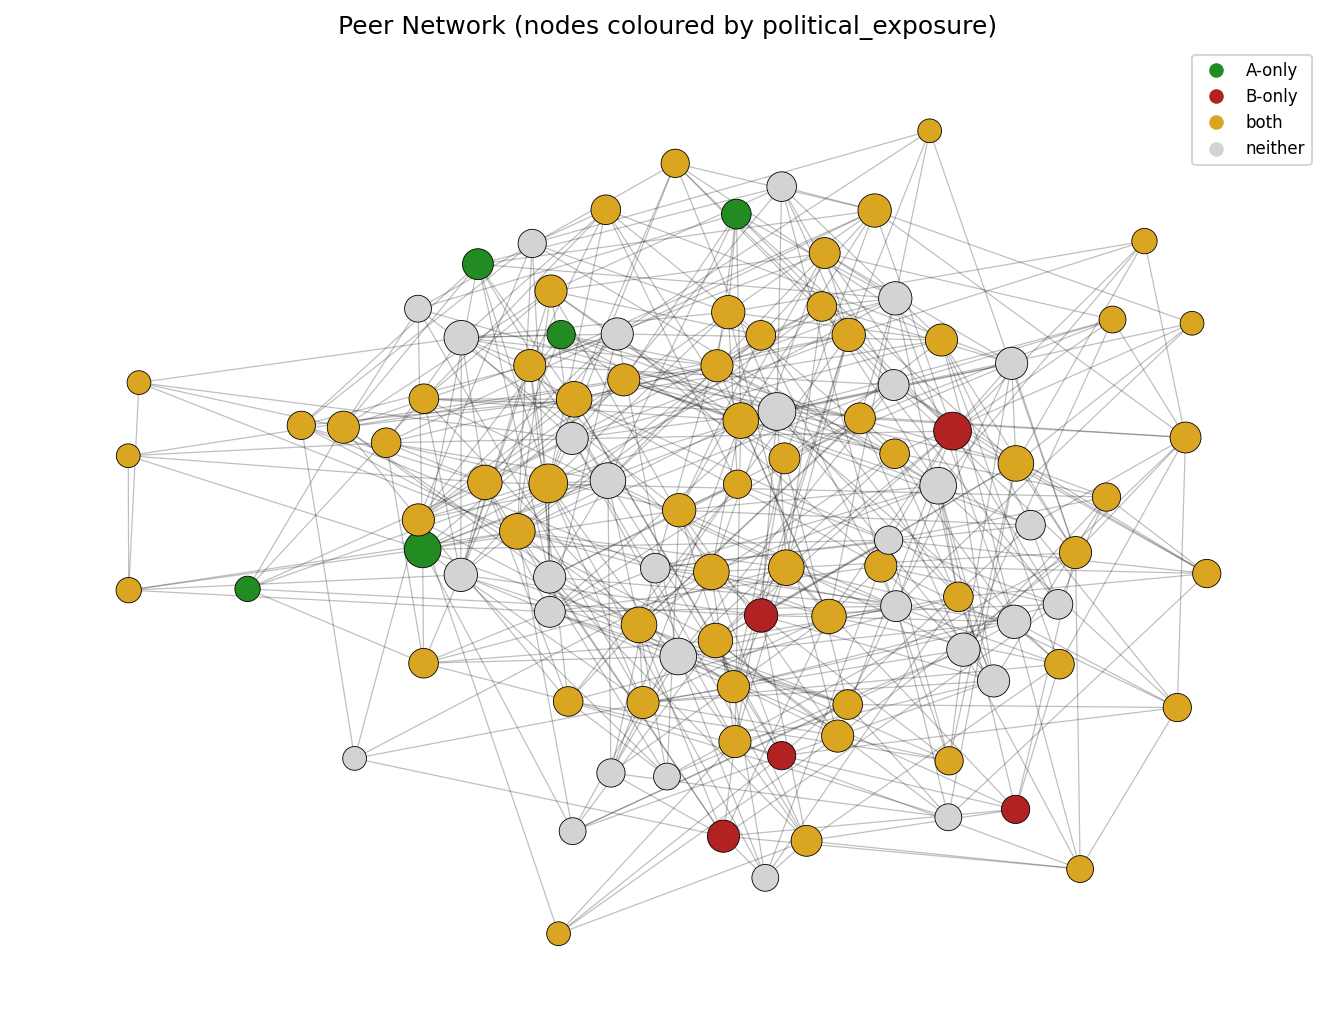
\includegraphics[width=0.8\textwidth]{figures/peer_network_exposure.png}
  \caption{Peer-messaging network for one reported run ($N=100$ citizen agents), with nodes coloured by assigned committed-minority exposure: the pro-climate side only (green), the sceptic side only (dark red), both sides (gold), or neither (grey). The graph is a two-block stochastic block model keyed on this exposure structure ($p_{\mathrm{intra}}=0.15$, $p_{\mathrm{inter}}=0.05$), but because the cross-cutting citizens who hear both sides and the disengaged citizens who hear neither together make up most of the population and are distributed across both blocks, no visible ideological clustering emerges: the network is only weakly sorted by exposure rather than a strict echo chamber.}
  \label{fig:sbm}
\end{figure*}

%\subsection{Daily phase loop}\label{subsec:phases}
Each simulated day has three message phases and one survey readout. Citizen AI agents
are exposed first to communication from committed minority groups (refer to
Figure~\ref{fig:gabm-framework}). Those who receive messages from both committed
minority groups can either receive first the pro-climate message and then the
anti-climate message or the other way round. The order of the messages varies randomly
day by day. After every exposure, they are asked to produce a short private reflection.
The citizen AI agents can then exchange peer messages (their climate policy reflections)
with $k$ randomly chosen neighbours. Those exposed to peer citizen communication write
then another brief reflection. The ordering of those phases (committed minority vs
citizen communication) can itself be changed as an experimental condition.

At the end of the simulated day, each citizen AI agents is asked to answer the original
six survey
questions on climate policies, taking the generated climate policy reflections into
account. The answers are recorded on the same $-3$ to $+3$ scale and an overall climate
policy opinion index is calculated.

We have implemented a debiasing prompt for the end-of-day survey, asking the citizen AI
agent under an anti-sycophancy instruction to explain its current view from the
persona's standpoint and convert these views then into survey responses. We experimented
with a third-person wording of the prompt, but this resulted in worse performance in our
prompt comparisons and was dropped. All prompt templates (reflection, survey, rationale)
are available in the SI file, Sec S2.3.

%extended thinking remains optional where the underlying model supports it. NOT SURE WHAT THIS MEANS
The model framework can run the simulated day loop in \emph{per-single-policy} mode,
where
one policy is studied in isolation, or in \emph{climate policy package} mode, where
the six-policy bundle is studied as a whole. Model features such as citizen population
size $N$, and the time horizon $T$ (e.g. how many simulated days are included in the
model run) can also be changed.

%\subsection{Day~0 anchoring}\label{subsec:anchor}

%The main control on initial conditions is how Day~0 is set. In \emph{LLM-survey} mode, the model answers the survey cold and those answers become the starting point. This reproduces the baseline-bias problem documented in prior work~\cite{argyle2023, santurkar2023, bisbee2024, manivannan2026} and is kept mainly as a control. In \emph{ground-truth} mode, the agent starts from the respondent's observed survey answers. In \emph{ground-truth-with-rationale} mode, which is used in the reported runs, the agent also generates a short first-person explanation for those seeded answers.

%This anchored mode gives the agent a narrative starting point without showing it a running numeric history of its own opinions. At the cohort level it has a simple consequence: the Day~0 mean equals the YouGov mean by construction, so any later movement is attributable to the simulated interactions rather than to the language model's prior over climate policy.

%\subsection{Memory and end-of-day survey readout}\label{subsec:debias}

%Each agent carries a tiered memory: the current day's reflections are available in full, the previous two days are kept verbatim, and older material is compressed into short daily summaries. We deliberately do not show the model a running table of its own past numeric scores. Earlier versions did this, and the result was too much self-consistency: agents tended to repeat their previous numbers rather than respond to the day's messages.

% End-of-day surveys use a two-step debiasing prompt. First, the agent is asked under an anti-sycophancy instruction to explain its current view from the persona's standpoint. In a second call, it converts that view into an A--G survey response. This is the survey path used in the results and evaluation sections. A third-person wording of the question performed worse in our prompt comparisons and was dropped; extended thinking remains optional where the underlying model supports it.

%%%%%%%%%%%%%%%%%%%%%%%%%%%%%%%%%%%%%%%%%%%%%%%%%%%%%%%%%%%%%%%%%%%%%%
%% 3. EXPERIMENTAL DESIGN AND MANIPULATIONS
%%%%%%%%%%%%%%%%%%%%%%%%%%%%%%%%%%%%%%%%%%%%%%%%%%%%%%%%%%%%%%%%%%%%%%
\section{Experimental design}\label{sec:levers}

The framework is built to support controlled experiments: starting from the same anchored
cohort, we change one design choice at a time and read off the resulting opinion
dynamics. Our question is what happens when the two committed minorities have unequal
resources and, in particular, whether the form the advantage takes matters. A resource
advantage can buy three different things, which we treat as three separable levers, and
we add a fourth experiment that pits two of them against each other at a fixed budget.
Unless stated otherwise, every experiment uses the same base configuration: $N=100$
citizen agents anchored to the YouGov subset, all six climate policies in package mode, a
seven-day horizon, the committed-minority exposure structure of
Section~\ref{subsec:network}, active peer exchange ($k=2$), and three random seeds; a
single local open-weight language model (Qwen3-14B) drives every generative step. Full
per-experiment settings are tabulated in the SI, and all four experiments are reported in
Section~\ref{sec:probes} and summarised in Table~\ref{tab:experiments}.

The first lever is broadcast reach: what share of its audience a committed minority
actually reaches with each broadcast. Each agent has its own reach parameter in $[0,1]$,
so we can compare symmetric exposure, where both sides reach the same share of citizens,
against asymmetric exposure, where one side reaches more. Because most citizens can hear
both sides (Section~\ref{subsec:network}), lowering one side's reach leaves those citizens
increasingly exposed only to the better-resourced competitor. Reach is run on the
stochastic block model network.

The second lever is broadcast frequency: how often each side speaks within a simulated
day, holding reach fixed for both. A better-resourced minority may not reach more citizens
but may ``flood the space'' by broadcasting more often. We vary the per-day broadcast
counts of the two sides (for example, two-to-one and three-to-one) while keeping the daily
audience unchanged. Frequency is also run on the stochastic block model.

The third lever, targeting, asks whether, at a fixed and limited reach, it matters whom
the under-resourced side spends that reach on. Holding the pro-climate side to a small
quarter of its audience, we vary only which citizens it keeps: a random quarter, the most
persuadable quarter, or the best-connected hubs. Targeting is run on a scale-free
(Barab\'asi--Albert) network, whose hubs give degree-based targeting something to aim at.

The fourth experiment holds the total advantage fixed and asks how it is best spent,
pitting reach against frequency at a matched budget of total impressions: the same number
of impressions delivered broad-and-shallow (more reach, fewer broadcasts) versus
narrow-and-deep (less reach, more broadcasts). If total exposure were all that mattered,
the two allocations would coincide.

Across all four experiments, the factors that are not the object of a given experiment,
message content, phase ordering, and, within an experiment, the network structure, are
held fixed or randomised so that the manipulated lever is the only systematic difference.
We do vary the network structure across experiments, and in a dedicated robustness check
(Section~\ref{subsec:eval}) we confirm that the reach result holds on scale-free and
small-world graphs as well.

%and the order of the within-day phases. In the current paper these choices are mostly held fixed so that the reported probes remain interpretable. Probe~1 uses the full daily loop; Probe~2 switches peer exchange off to keep the structural comparison simple, but the result of interest is still the ordering induced by reach asymmetry.

%\subsection{Scale, scope, and what is left for later}\label{subsec:levers-population}

%Population size $N$, simulation horizon $T$, and policy scope determine what kind of claim a run can support. The framework can run one policy
%at a time or the full six-policy package, and it can be applied to subgroups of the YouGov panel rather than only to mixed cohorts. It can also, in principle, vary the effective size of the competing minorities by changing the sample or reweighting the panel, which is important for the tipping-style questions that motivate this broader research programme~\cite{centola2018}.

%These choices matter because they separate a proof of operation from a substantive test. The runs in Section~\ref{sec:probes} use small cohorts and short horizons, which are enough to show that the framework runs end to end and that one manipulation registers a signal, but not enough to support strong claims about long-run dynamics or tipping. Across the reported runs, the only lever treated as a substantive experimental manipulation is broadcast reach asymmetry. The rest of the design space defines the next set of experiments rather than claims made here.

%%%%%%%%%%%%%%%%%%%%%%%%%%%%%%%%%%%%%%%%%%%%%%%%%%%%%%%%%%%%%%%%%%%%%%
%% 4. RESULTS
%%%%%%%%%%%%%%%%%%%%%%%%%%%%%%%%%%%%%%%%%%%%%%%%%%%%%%%%%%%%%%%%%%%%%%
\section{Results}\label{sec:probes}

% =====================================================================
% RESULTS SECTION — draft-45 program: four resource-advantage experiments
% (N=100, Qwen3-14B, 7-day, package mode, 3 seeds), fronted by a
% fit-for-purpose evaluation. Internal labels only: evaluation = Tier P/1/2/3;
% the four experiments = Bites 1-4 (reach / frequency / targeting / iso).
%   Every number below is recomputed from the raw runs and verified in the
%   provenance notebooks notebooks/45_evaluation_audit.ipynb (32 checks pass)
%   and notebooks/46_experiments_audit.ipynb; machine-readable outputs in
%   paper/tables/ (audit_evaluation.csv, audit_experiments.csv,
%   table1_experiments.csv). Do NOT cite docs/result_report.md in the paper —
%   cite the SI / the paper/tables CSVs.
% Metric contract (main text only): mean package index on -3..+3; support/
% oppose shares (%); within-person difference in scale points with 95% CI;
% Spearman rho + signed bias for the evaluation; "same sign in every seed"
% for reliability. DiD / Cohen dz / ANCOVA / ceiling rulers -> SI.
% =====================================================================

A single committed minority can, under the right conditions, pull a much larger
population towards its position. Real advocacy, however, rarely takes place between one
minority and a passive majority: competing minorities push in opposite directions, and
they almost never do so with equal resources. The question this section addresses is
therefore not whether a committed minority can move the majority, but what
happens when two of them compete with unequal resources and, in particular, whether
the form of a resource advantage decides who prevails. A larger budget can buy
different things: it can reach more citizens (reach), broadcast more often
(frequency), or aim a limited broadcast more cleverly (targeting). We ask
whether these forms are interchangeable, or whether what the resources buy
matters as much as how much there is.

We report four experiments (N=100 citizen agents, seven simulated days, all six
climate policies, Qwen3-14B, three random seeds per condition), each isolating one form
of a resource advantage; together with the evaluation that precedes them, they rest on
sixty-nine independent simulations spanning three social-network topologies
(stochastic-block, scale-free and small-world) and two language-model families. Before
the substantive results we present a fit-for-purpose evaluation of the instrument itself. A note on interpretation governs everything that
follows: we make no claim that the model reproduces real-world opinion dynamics. Our
evaluation targets internal validity (that the
difference we measure between two conditions is really caused by the lever we changed)
and algorithmic fidelity (that the machinery does what we intend), not external validity
(that the same result would hold in the real world), which, we argue, is an open
problem no current GABM has solved. Every result below is a relative,
within-model, directional comparison.

Throughout, the outcome is each citizen's package index: the average of their six
climate-policy answers on a $-3$ (strongly oppose) to $+3$ (strongly support) scale, and
its mean across the population. Because every condition pins each agent's Day~0 opinion
to the same observed survey value, the effect of a manipulation is simply a
within-person difference in final opinion: how much more (in scale points, with a
95\% confidence interval) the same citizen ends up supporting climate policy under one
condition than another. This paired difference has a standard formal justification,
which we give in the SI (together with the accompanying effect sizes and
ceiling-robust rulers); in the main text we keep to the plain scale-point difference
and, where it aids intuition, the share of citizens supporting versus opposing.

\subsection{Does the instrument work? A fit-for-purpose evaluation}\label{subsec:eval}
% FIGURE E1 (TODO): evaluation summary — persona signal (rho), rank fidelity, signed bias.

Before asking what the levers do, we ask whether the instrument does what it is supposed
to. We frame this as an explicit, reusable evaluation protocol, itself a contribution,
built around four instrument questions rather than a claim of real-world validation.

Does it read the persona it is given? Each agent is initialised from a real
YouGov respondent, and its Day~0 answers track that respondent's actual survey answers
closely (Spearman rank correlation $\rho \approx 0.62$ on the package index, that is,
the model keeps citizens in nearly the same order as the real survey). When the personas
are permuted so that each agent is scored against the wrong respondent, this correlation
collapses to near zero; an agent handed a stranger's persona adopts the stranger's
opinions rather than its own, and stripping the persona away entirely collapses the
spread of opinions to a near-uniform response (SI). The instrument is genuinely reading
the input it is handed rather than producing a generic response.

Does it respond to the lever? Turning up one side's reach produces a clear,
correctly-signed response: the same citizen ends up about $+0.42$ package-index points
more pro-climate when the pro-climate minority reaches more citizens than when the
sceptic minority does (95\% CI $[+0.34, +0.51]$). A silent no-broadcast placebo
condition barely moves (the two sides push $+0.32$ up and $-0.10$ down relative to it),
confirming that the broadcasts, not the mere passage of simulated time, do the work.

Is the effect real, or an artefact of the bounded scale? Because the $-3$ to $+3$
scale has a ceiling, agents near the top cannot move further up, which could manufacture
an apparent asymmetry. Re-expressing the same final opinions on ceiling-robust rulers
(SI, Table~S8) leaves the effect essentially uniform across the opinion spectrum: an
apparent tilt at the top of the scale was the ceiling, not a genuine interaction.

Is it reliable across choices we could have made differently? The reach effect is
robust across social-graph structure (three network topologies give same-signed, highly
significant differences of $+0.34$ to $+0.42$, replicated over three seeds) and across
the language model itself (re-running on Llama-3.1-8B reproduces a same-signed, strongly
significant difference). Notably, that second model is a demonstrably worse
simulator: it keeps citizens in the right order only weakly ($\rho \approx 0.46$) and
reads systematically low rather than high, yet the contrast survives, because a
within-person difference cancels each model's common-mode error. The difference-engine
design is credible precisely because the effect persists even on a model that gets
absolute opinions wrong.

\subsection{Reaching more citizens moves the majority}\label{subsec:bite-reach}
% FIGURE 1 (TODO): reach dose-response — within-person difference vs reach gap.
% Numbers verified in paper/tables/ (NB 46); seven-day ladder, 15 of 18 runs (placebo pending).

The first form of advantage is reach: speaking to more people. On the seven-day horizon
we sweep a graded reach ladder, throttling one side to a half or a quarter of its
audience while the other keeps full reach, and compare against symmetric ($1{:}1$)
exposure. Widening the reach gap in favour of one side produces a same-signed, graded
shift of the majority toward that side. At the widest gap, when the pro-climate minority
reaches four times as many citizens as the sceptic minority, the same citizen ends up
about $+0.35$ package-index points more pro-climate (95\% CI $[+0.27, +0.44]$), same sign
in all three seeds; halving the reach gap roughly halves the shift ($+0.29$), an internal
dose-response, and the ladder is monotone in the gap, plateauing once the pro-climate
side saturates the top of the scale. Both sides contribute: relative to symmetric
exposure, a pro-climate reach edge lifts opinion ($+0.15$) and a sceptic reach edge
lowers it ($-0.21$). This whole-population figure is diluted by the citizens who hear
only one side; among the majority who hear both sides the shift is larger, about $+0.45$.
The effect is broad across all six individual policies rather than driven by any single
one (SI), and it agrees with the five-day reach contrast on which the evaluation above is
built (Section~\ref{subsec:eval}; $+0.42\ [+0.34, +0.51]$), which additionally validates
it across network topology and language model. Reaching more citizens moves the majority.

\subsection{Broadcasting more often also moves the majority, but by less}\label{subsec:bite-freq}
% FIGURE 2 (TODO): frequency dose-response — 2:1 vs 3:1 within-person difference.

The second form of advantage is frequency: speaking more often to the same audience.
Holding reach equal for both sides, letting one minority broadcast twice as often as the
other shifts the same citizen $+0.16$ package-index points toward the louder side (95\%
CI $[+0.09, +0.23]$); widening the gap to three-to-one nearly doubles the shift to
$+0.28$ ($[+0.20, +0.36]$), an internal dose-response. As with reach, the effect
concentrates among the majority who hear both streams ($+0.15$ at two-to-one, $+0.34$ at
three-to-one), the signature of genuine persuasion rather than a passage-of-time
artefact, and is same-signed in every seed (though its magnitude varies across seeds, so
we report direction rather than a precise size). The share of citizens supporting
climate policy rises from about 78\% to 83\% as the pro-climate side grows louder.
Frequency is thus a real second ``more resources'' lever, but a weaker one: a
three-to-one frequency advantage ($+0.28$) moves opinion less than a four-to-one reach
advantage ($+0.35$). That reach and frequency are separable and produce different
effect sizes is itself something a classical model, which folds them into a single
influence weight, cannot show.

\subsection{Whom the message reaches does not substitute for how much it is broadcast}\label{subsec:bite-target}
% FIGURE 3 (TODO): targeting-mode comparison (random / persuadable / degree), null.

The third form of advantage is targeting: at a fixed, limited reach, choosing
whom to speak to. We throttled the under-resourced (pro-climate) side to a
quarter of its audience on a hub-structured network and varied only whom it kept: a
random quarter, the most persuadable quarter (citizens with the weakest prior
convictions), or the best-connected hubs. None beat random: targeting the persuadable
rather than a random quarter changes the outcome by $+0.04$ points (not significant),
targeting hubs by $+0.03$ (not significant), and neither sign is stable across seeds.
The lever fired exactly as designed (the persuadable mode did keep the low-conviction
citizens and the hub mode did keep the well-connected ones, SI), so this is a genuine
null, not a broken manipulation. Indeed, a framework that returned an effect from
every manipulation would be suspect; that reach and frequency register while
targeting does not is evidence the instrument discriminates. The honest reading is
bounded: at a quarter reach over seven days, whom the under-resourced side aims at does
not measurably change the majority's opinion; the point estimates weakly favour smart
targeting but are neither significant nor sign-stable. Two features of our design further
bound the hub result in particular: every citizen relays messages to the same small
number of peers each day ($k=2$), regardless of how well connected they are, so a
targeted hub cannot pass its shifted opinion to more neighbours than anyone else; and
hub-targeting's payoff, network spillover, may in any case be too slow to accumulate
over seven days. We therefore read this as no measurable effect under the present peer
mechanism and horizon, not as evidence that targeting is ineffective in general; a
degree-proportional relay rule and a longer horizon are the natural re-tests.

\subsection{Reach and frequency are not interchangeable}\label{subsec:bite-iso}
% FIGURE 4 (TODO): iso-impression — breadth (depth2) vs depth (depth4) at equal impressions.

The three experiments above vary the amount or placement of a resource advantage. The final
experiment holds the total advantage fixed and asks how it is best spent. We gave the
pro-climate side a fixed budget of total impressions and allocated it two ways:
broad-and-shallow (reach half the audience, broadcast twice a day) versus
narrow-and-deep (reach a quarter, broadcast four times a day). If total exposure were
the only thing that mattered, the two allocations would coincide. They do not. The
broad-and-shallow allocation leaves the same citizen $+0.12$ package-index points more
pro-climate (95\% CI $[+0.03, +0.21]$), same sign in all three seeds, and larger among
the majority who hear both sides ($+0.20$). The margin is modest but reliable: total
impressions is not a sufficient statistic for persuasion, and spreading a fixed
budget wide beats stacking it deep. Reach and frequency are therefore not freely
interchangeable.

\subsection{What the resources buy}\label{subsec:synthesis}

Taken together, the four experiments form a ladder (Table~\ref{tab:experiments}). Reach
is the strongest and most thoroughly validated lever ($\approx +0.35$ on the graded
seven-day ladder, consistent with the $+0.42$ five-day validation), frequency a real but
weaker one ($+0.16$ to $+0.28$), and targeting registers no measurable effect ($\approx
0$) within the
tested range; and at a fixed impression budget, breadth beats depth. The form of
a resource advantage, not merely its size, shapes who moves the majority, and the
forms are not interchangeable. For competing committed minorities this reframes the
question from ``who has more resources'' to ``what those resources buy'': volume moves
opinion, placement (within the tested range and horizon) does not, and a given volume
does more spread wide than stacked deep. Each of these contrasts rests on holding apart
levers that a classical committed-minority model collapses into a single influence
weight: the separability that a generative agent-based model uniquely affords, and
the methodological payoff of the approach.

% TABLE 1 --- verified against paper/tables/table1_experiments.csv (NB 46).
\begin{table*}[t]
\centering
\small
\caption{The four resource-advantage experiments. Each effect is the within-person
difference in the final package index (on the $-3$ to $+3$ scale), pooled over three
seeds; a positive value favours the pro-climate side. ``Among those who hear both
sides'' is the same difference restricted to the majority exposed to both broadcast
streams. Values are recomputed from the raw runs and verified in the provenance
notebooks (SI). n.s., not significant.}
\label{tab:experiments}
\begin{tabular}{@{}p{2.1cm}p{3.0cm}p{4.6cm}p{2.3cm}p{2.2cm}c@{}}
\toprule
Experiment & What the advantage buys & Whole-population effect (95\% CI) & Among those who hear both sides & Reliability & $n$ \\
\midrule
Reach & reach more citizens & $+0.35\ [+0.27, +0.44]$ & $+0.45$ & same sign, 3/3 seeds & 15 \\
Frequency & broadcast more often & $+0.16\ [+0.09, +0.23]$ at 2:1; $+0.28\ [+0.20, +0.36]$ at 3:1 & $+0.15$ / $+0.34$ & same sign, 3/3 seeds & 12 \\
Targeting & aim a limited broadcast & $+0.04$ (n.s.); $+0.03$ (n.s.) & $\approx 0$ (n.s.) & mixed sign & 9 \\
Breadth vs depth & spend a fixed budget wide or deep & $+0.12\ [+0.03, +0.21]$ & $+0.20$ & same sign, 3/3 seeds & 6 \\
\bottomrule
\end{tabular}
\end{table*}


\section{Discussion} \label{sec:discuss}

\subsection{Reflection on results}

The program does more than register a single signal: it separates the forms of a
resource advantage and shows they are not equivalent. Reach, speaking to more citizens,
is the strongest and most thoroughly validated lever; broadcasting more often is a real
but weaker one; and, at a fixed impression budget, spreading a message wide beats
stacking it deep. Targeting a shrunken broadcast at the persuadable or the
well-connected, by contrast, produces no measurable population shift within the tested
range. Read together, these four experiments answer the question that motivates the
paper: when two committed minorities compete with unequal resources, the form of the
advantage, not merely its magnitude, shapes who moves the majority.

This separability is the methodological payoff of a generative agent-based model.
Classical committed-minority models collapse reach, frequency, targeting, and message
content into a single abstract influence weight; because our agents process
natural-language messages against personas, the framework can hold these apart and
estimate their effects independently. We do not claim the approach is superior to
classical agent-based models, and we deliberately avoid a head-to-head comparison, which
is out of scope here. The claim is narrower and complementary: a GABM makes a class of
questions, about what a resource advantage buys, addressable that a fixed-rule model
cannot express. The evaluation protocol we report (reading the persona, responding to
the lever, ruling out a scale artefact, and replicating across graph and model) is
itself a reusable contribution for vetting this class of model.

\subsection{Limitations}

We restate, in its strongest form, the caveat that bounds everything above: we make no
claim that the model reproduces real-world opinion dynamics. Our evidence establishes
internal validity and algorithmic fidelity, not external validity, and we would argue
that establishing external validity for a GABM is an open problem the field has not
solved. Every effect we report is a relative, within-model, directional comparison, and
should be read as such.

The substantive results rest on a cohort of $N=100$ agents, our intended design size and
sufficient for these within-model contrasts, over a short horizon of seven days; this is
enough to identify directional contrasts, but the short horizon means we make no claims
about long-run stability, rebound, or tipping. The reach effect is validated across social
graphs and a second language model (Section~\ref{subsec:eval}); what remains outstanding
is only its finer dose-response, the graded reach ladder, so the values reported here
will be refined rather than overturned by those runs. The language model carries a known
pro-climate level bias (larger on the cost-framed Carbon tax and Climate compensation
items); we neutralise it by reporting within-person paired differences against a common
Day~0 anchor and a silent placebo, so the common-mode bias cancels and we never make an
absolute-level claim. Because LLM outputs are stochastic, we run three seeds wherever
possible and report sign-stability alongside the effect; magnitudes vary across seeds, so
we lead with direction rather than a precise number. The cross-model replication uses a
single seed and therefore supports a directional, within-sample claim only, not a
cross-draw magnitude claim. Finally, the package index is our primary outcome; per-policy
breakdowns are reported in the SI.

\subsection{Future works}

The results point to several natural next steps that the framework already supports.

The clearest limitation is horizon. Extending from seven to roughly thirty simulated
days is the prerequisite for the tipping-style questions, threshold-like cascades under
competing minorities, that motivate the broader programme; it is also the most likely
setting in which the targeting null would resolve, since hub-targeting's payoff is
network spillover, which a short horizon may be too brief to accumulate.

Resolving the reach dose-response is the next step. Completing the graded reach ladder,
holding the cohort at our target of $N=100$, would let the reach effect be characterised
as a graded quantitative property with a cross-draw magnitude, rather than the
directional contrast reported here.

Model breadth would further strengthen the reliability claim. The reach contrast already
replicates on a second model family; adding a third, together with a seed sweep, would
license a cross-model magnitude comparison rather than a directional one.

Message content is a further, untested lever. In the reported runs each side draws its
broadcasts from a fixed pool of synthetic messages grounded in real party
communications; systematically varying that content, its framing, its emotional
intensity, and its provenance (how much is verbatim-real rather than synthetic), would
test whether persuasive
content constitutes a separable resource lever alongside reach and frequency
(Section~\ref{subsec:political}).

Finally, several design levers remain fixed or randomised here, phase ordering, peer
fan-out $k$, cohort composition, and committed-minority size, and each is a candidate
manipulation for isolating additional drivers of competing opinion dynamics.

\section*{Additional information}

Full details of the model architecture, data preparation, prompt design, and calibration
are provided in the Supplementary Information (SI). Section~S1 describes the YouGov
survey data, the analytic filtering that yields the $N=1{,}483$ model-ready subset, and
the six climate-policy items used as outcome measures (Tables~S1 and~S2).

Section~S2 reproduces the citizen persona construction with two worked examples, the
composition and real-source provenance of each side's fixed message pool, and the exact
prompt templates used in all reported runs, including the
two-step debiased end-of-day survey and the memory-compression routine.

Section~S3 documents the runtime pipeline: population instantiation, the rule-based
audience assignment logic (Table~S3), stochastic block model construction, the Day~0
anchoring modes, and the within-day phase execution order. Tables~S4--S7 summarise the
configuration settings, Day~0 baselines, and per-condition outcomes for the experiments
reported in Section~\ref{sec:probes}.

The evaluation of the survey path is reported in Section~S4. Section~S5 outlines further
extension paths, including parallelisation, cognitive architecture improvements,
persona-faithfulness refinements, and local-model deployment.

% \subsection{Limitations}

% The reported runs are small. Results use $N=30$ citizens over four days under three random seeds. The paper also uses one model stack per role (GPT-5-mini for reflections, peer messages, and political broadcasts; Claude Sonnet for end-of-day surveys), one policy domain, and a two-political-agent abstraction. Those choices are only enough to test whether the framework runs end-to-end and whether one manipulation registers a signal.

% We do not yet know whether opinion change under peer messaging matches how people respond to peer influence outside the model; we only know that peer exchange produces interpretable trajectories in the current runs. We also do not yet know how much the tiered memory architecture distorts late-run dynamics over longer horizons, because earlier days are compressed into summaries rather than preserved in full. 

% \subsection{Future Works}

% The framework is now far enough along to support a more structured next phase. The most useful next steps fall into three groups: robustness and scale, mechanism tests, and longer-term development.

% The immediate priority is to extend the experiment across a larger set of replications and population size for robustness. In addition, we are interested in policy package analysis, which combines the six discussed policies, for index-level analysis, rather than a single policy study.
%%%%%%%%%%%%%%%%%%%%%%%%%%%%%%%%%%%%%%%%%%%%%%%%%%%%%%%%%%%%%%%%%%%%%%
%% 6. SCOPE AND LIMITATIONS
%%%%%%%%%%%%%%%%%%%%%%%%%%%%%%%%%%%%%%%%%%%%%%%%%%%%%%%%%%%%%%%%%%%%%%
%\section{Scope and limitations}\label{sec:limits}

%This paper should be read as a proof of operation for one framework configuration. It is not a population estimate of UK opinion change, and it is not a tipping claim. The main constraints fall into three groups: scope, validity risks already addressed, and validity risks still open.

%\subsection{Current scope}\label{subsec:limits-scope}

%The reported runs are deliberately small. Probe~1 uses $N=30$ citizens over seven days under one random seed, and Probe~2 uses $N=30$ over four days in three reach conditions, with the reported ordering checked across three independently sampled cohorts and the figures showing one of them. Wall time is still dominated by sequential language-model calls, so larger cohorts and longer horizons were out of scope here. The paper also uses one model stack per role (GPT-5-mini for reflections, peer messages, and political broadcasts; Claude Sonnet for end-of-day surveys), one policy domain, and a two-political-agent abstraction. Those choices are enough to test whether the framework runs end to end and whether one manipulation registers a signal. They are not enough to support population-level claims, cross-model claims, or richer multi-actor dynamics.

%\subsection{Addressed and open validity risks}\label{subsec:limits-validity}

%Two important risks are already handled directly. First, initialisation bias is controlled by the Day~0 anchor in \S\ref{subsec:anchor}: the cohort starts from observed YouGov answers rather than opinions generated from scratch by a language model.
%Second, survey-path bias is measured rather than assumed away: Section~\ref{sec:grounding} shows that the evaluation path reads persona, behaves reasonably on four of the six policies, and retains a known positive bias on Carbon tax and Climate compensation.

%Two further risks remain open. We do not yet know whether opinion change under peer messaging matches how people respond to peer influence outside the model; we only know that peer exchange produces interpretable trajectories in the current runs. We also do not yet know how much the tiered memory architecture distorts late-run dynamics over longer horizons, because earlier days are compressed into summaries rather than preserved in full. These are measurement targets for the next phase, not background caveats.

%\subsection{What would be needed for a tipping claim}\label{subsec:limits-tipping}

%The current paper does not test for tipping. Here, tipping would mean a threshold-like cascade in which a small change in exposure or alignment produces self-reinforcing population change. Detecting that kind of behaviour would require longer horizons, replicated seeds, sweeps over committed-minority size, and an explicit rule for identifying a tipping event under noise. None of that evidence is presented here. The point of the next stage is to test systematically whether this framework can produce that kind of behaviour, and under what conditions.

%%%%%%%%%%%%%%%%%%%%%%%%%%%%%%%%%%%%%%%%%%%%%%%%%%%%%%%%%%%%%%%%%%%%%%
%% 7. FUTURE WORK AND OPEN QUESTIONS
%%%%%%%%%%%%%%%%%%%%%%%%%%%%%%%%%%%%%%%%%%%%%%%%%%%%%%%%%%%%%%%%%%%%%%
%\section{Future work and open questions}\label{sec:roadmap}

%The framework is now far enough along to support a more structured next phase. The most useful next steps fall into three groups: robustness and scale, mechanism tests, and longer-term development.

%\subsection{Robustness and scale}\label{subsec:roadmap-probes}

%The immediate priority is extension beyond the current three-replication check. Probe~2 should next be run on at least one additional policy and across a larger set of replications, so that the reach-asymmetry ordering can be treated as a robust property of the framework rather than of one short schedule. The next scaling step is to extend horizon and population size once intra-phase parallelisation reduces wall time per simulated day. Those two changes are the minimum required before stronger claims about stability, rebound, or cascade-like behaviour become credible.

%\subsection{Mechanism tests enabled by the current design}\label{subsec:roadmap-mechanisms}

%The current framework already supports a broader mechanism programme than this paper uses. The most direct next manipulations are committed-minority size, persuasive-capability asymmetry, phase ordering, peer fan-out, and more or less cross-cut exposure in the network. It can also support content-focused tests, such as message framing, single-policy versus package-level runs, and subgroup-specific responses across different cohort compositions. Taken together, these levers move the framework from proof of operation toward controlled comparisons about which features of communication actually drive change.

%\subsection{Longer-term development and useful input}\label{subsec:roadmap-feedback}

%Longer-term goals are larger populations, longer horizons, richer elite competition, and stronger checks on memory and peer influence. Plausible extensions include more than two political agents, explicit media or platform mediation, dynamic network rewiring, and cross-model comparison of the survey path. The most useful suggestions at this stage are pragmatic ones: which robustness check should come first, which existing lever is most likely to change the conclusions, and what empirical comparison would most increase confidence before stronger claims about cascade dynamics or generalisation are made.
\clearpage
%%%%%%%%%%%%%%%%%%%%%%%%%%%%%%%%%%%%%%%%%%%%%%%%%%%%%%%%%%%%%%%%%%%%%%
%% BACKMATTER
%%%%%%%%%%%%%%%%%%%%%%%%%%%%%%%%%%%%%%%%%%%%%%%%%%%%%%%%%%%%%%%%%%%%%%
\backmatter

% \bmhead{Acknowledgements}
% % TODO

% \section*{Declarations}

% \begin{itemize}
% \item \textbf{Funding}: % TODO
% \item \textbf{Conflict of interest}: The authors declare no competing interests.
% \item \textbf{Ethics approval}: Secondary analysis of an existing YouGov survey panel; no new human-subjects data collected.
% \item \textbf{Data availability}: % TODO
% \item \textbf{Code availability}: Source code available at \url{https://github.com/} % TODO add repo URL
% \item \textbf{Author contribution}: % TODO
% \end{itemize}

%%%%%%%%%%%%%%%%%%%%%%%%%%%%%%%%%%%%%%%%%%%%%%%%%%%%%%%%%%%%%%%%%%%%%%
%% BIBLIOGRAPHY
%%%%%%%%%%%%%%%%%%%%%%%%%%%%%%%%%%%%%%%%%%%%%%%%%%%%%%%%%%%%%%%%%%%%%%
\bibliography{references}

\end{document}

